%--------------------------------------------------
%--------------------------------------------------

\subsection{Conexidad}

\paragraph{\textbf{Teorema.}}
Sea $A\subseteq X$ conexo.  
Si $A\subseteq B \subseteq \overline{A}$, entonces $B$ es conexo.

\paragraph{\textbf{Demostración.}}
Supongamos que $B$ se descompone en $B=C\sqcup D$, donde $C$ y $D$ son abiertos disjuntos y no vacíos.  
Intersectando con $A$ se obtiene
\begin{align*}
A\subseteq C \quad \lor \quad A\subseteq D .
\end{align*}
Además,
\begin{align*}
A=(C\cap A)\cup(D\cap A),
\end{align*}
y como $A$ es conexo y $(C\cap A)\neq\varnothing$ o $(D\cap A)\neq\varnothing$, concluimos que $A\subseteq C$ o $A\subseteq D$.  
Sin pérdida de generalidad, supongamos $A\subseteq C$.  
Tomando clausuras,
\begin{align*}
\overline{A}\subseteq\overline{C}.
\end{align*}

Sea $x\in\overline{C}\cap D$.  
Dado que $D\subseteq B$ y $D=U\cap B$ para algún abierto $U\subseteq X$ con $x\in U$, se cumple
\begin{align*}
U\cap C\neq\varnothing .
\end{align*}
Por tanto,
\begin{align*}
B\cap(U\cap C)=U\cap(B\cap C)=U\cap C\neq\varnothing ,
\end{align*}
pues $B\supseteq C$. Luego
\begin{align*}
(B\cap U)\cap C=D\cap C\neq\varnothing ,
\end{align*}
Lo cual es una contradicción, ya que $C$ y $D$ son disjuntos. Por lo que $\overline{C}\cap D=\varnothing$. Pero $A\subseteq C$, así que
\begin{align*}
\overline{A}\cap D = \varnothing .
\end{align*}

Como $B\cap D=\varnothing\subseteq \overline{A} \cap D =\varnothing$, se deduce $D=\varnothing$, contradicción. \hfill$\square$




%--------------------------------------------------
%  Continuidad y conexión
%--------------------------------------------------

\paragraph{\textbf{Teorema.}}
Si $f\colon X\to Y$ es continua y $X$ es conexo, entonces $f(X)$ es conexo.

\paragraph{\textbf{Demostración.}}
Supongamos que $f(X)=A\cup B$, donde $A$ y $B$ son abiertos, disjuntos y no vacíos. Entonces $f^{-1}(A)\cup f^{-1}(B)$ es una separación de $X$ (figura a continuación), contradiciendo que $X$ es conexo. \hfill$\square$

\begin{center}
  \shorthandoff{>}
  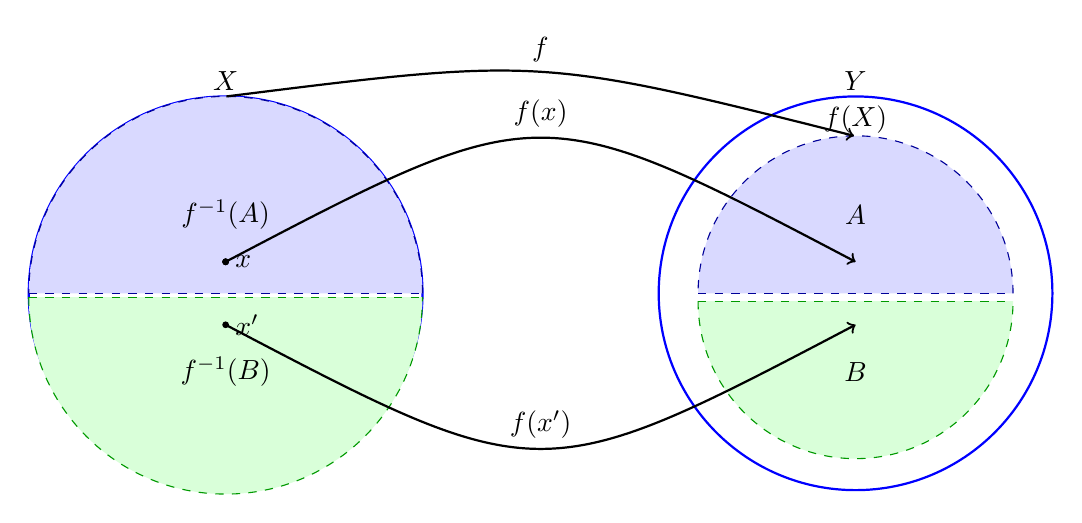
\begin{tikzpicture}
      % Set x
       \draw[blue, thick] (-4,0) circle (2.5cm);
       \node at (-4,2.7) {$X$};

       \fill[green!15] (-4,-0.05) ++(-2.5cm,0cm) arc[start angle=180, end angle=360, x radius=2.5cm, y radius=2.5cm] -- cycle;
       \draw[green!60!black, dashed] (-4,-.05) ++(-2.5cm,0cm) arc[start angle=180, end angle=360, x radius=2.5cm, y radius=2.5cm];
       \draw[green!60!black, dashed] (-6.5,-.05) -- (-1.5,-.05);
       \node at (-4,-1) {$f^{-1}(B)$};

       \filldraw[black] (-4,-.4) circle (1pt) node[ right] {$x'$};

 
       % Half-ellipse representation of f(X)
       \fill[blue!15] (-4,0) ++(2.5cm,0cm) arc[start angle=0, end angle=180, x radius=2.5cm, y radius=2.5cm] -- cycle;
       \draw[blue!60!black, dashed] (-4,0) ++(2.5cm,0cm) arc[start angle=0, end angle=180, x radius=2.5cm, y radius=2.5cm];
       \draw[blue!60!black, dashed] (-6.5,0) -- (-1.5,0);
       \node at (-4,1) {$f^{-1}(A)$};

      % Draw the set U in X
      % \node at (-2.5,0) {$f^{-1}(V)$};
    
      
      % Set Y
      \draw[blue, thick] (4,0) circle (2.5cm);



      % Point x inside the set
      \filldraw[black] (-4,.4) circle (1pt) node[right] {$x$};


      % Set Y
      \node at (4,2.7) {$Y$};
      % Image f(X) inside Y
      %  \fill[green!15] (4,0) ellipse (1.7cm and 2.0cm);
      %  \draw[green!60!black, thick] (4,0) ellipse (1.7cm and 2.0cm);
      %  \node at (4.2,2.2) {$f(X)$};
      % Ambient space
       % Half-ellipse representation of f(X)
      \fill[green!15] (4,-0.1) ++(-2cm,0cm) arc[start angle=180, end angle=360, x radius=2cm, y radius=2.0cm] -- cycle;
      \draw[green!60!black, dashed] (4,-.1) ++(-2cm,0cm) arc[start angle=180, end angle=360, x radius=2cm, y radius=2.0cm];
      \draw[green!60!black, dashed] (2,-.1) -- (6,-.1);
      \filldraw[black] (-4,.4) circle (1pt);

      \node at (4,-1) {$B$};

      % Half-ellipse representation of f(X)
      \fill[blue!15] (4,0) ++(2cm,0cm) arc[start angle=0, end angle=180, x radius=2cm, y radius=2.0cm] -- cycle;
      \draw[blue!60!black, dashed] (4,0) ++(2cm,0cm) arc[start angle=0, end angle=180, x radius=2cm, y radius=2.0cm];
      \draw[blue!60!black, dashed] (2,0) -- (6,0);
      \filldraw[black] (-4,.4) circle (1pt);
      \node at (4,1) {$A$};
      \node at (4,2.2) {$f(X)$};
       % Ambient space

      
  

      \draw[->, thick] (-3.99,2.5) .. controls (0,3) .. (3.98,2) node[midway, above] {\(f\)};

      \draw[->, thick] (-4,.4) .. controls (0,2.5) .. (4,.4) node[midway, above] {\(f(x)\)};


      % Arc arrow representing the function f^-1 from V to U
      \draw[->, thick] (-4,-.4) .. controls (0,-2.5) .. (4,-.4) node[midway, above] {\(f(x')\)};

  \end{tikzpicture}
  \shorthandon{>}
\end{center}



\begin{center}
  \shorthandoff{>}
  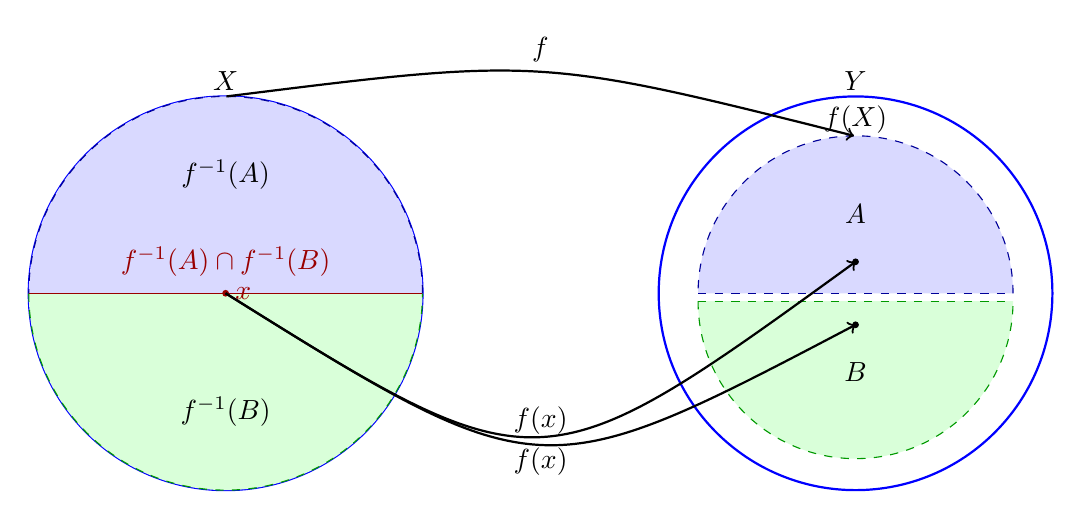
\begin{tikzpicture}
      % Set x
       \draw[blue, thick] (-4,0) circle (2.5cm);
       \node at (-4,2.7) {$X$};

       \fill[green!15] (-4,0) ++(-2.5cm,0cm) arc[start angle=180, end angle=360, x radius=2.5cm, y radius=2.5cm] -- cycle;
       \draw[green!60!black, dashed] (-4,0) ++(-2.5cm,0cm) arc[start angle=180, end angle=360, x radius=2.5cm, y radius=2.5cm];
       \node at (-4,-1.5) {$f^{-1}(B)$};

 
       % Half-ellipse representation of f(X)
       \fill[blue!15] (-4,0) ++(2.5cm,0cm) arc[start angle=0, end angle=180, x radius=2.5cm, y radius=2.5cm] -- cycle;
       \draw[blue!60!black, dashed] (-4,0) ++(2.5cm,0cm) arc[start angle=0, end angle=180, x radius=2.5cm, y radius=2.5cm];
       \node[red!60!black] at (-4,.4) {$f^{-1}(A) \cap f^{-1}(B)$};

       \node at (-4,1.5) {$f^{-1}(A)$};

       \draw[red!60!black] (-6.5,0) -- (-1.5,0);
       \filldraw[red!60!black] (-4,0) circle (1pt) node[ right] {$x$};


      % Draw the set U in X
      % \node at (-2.5,0) {$f^{-1}(V)$};
    
      
      % Set Y
      \draw[blue, thick] (4,0) circle (2.5cm);


      % Set Y
      \node at (4,2.7) {$Y$};
      % Image f(X) inside Y
      %  \fill[green!15] (4,0) ellipse (1.7cm and 2.0cm);
      %  \draw[green!60!black, thick] (4,0) ellipse (1.7cm and 2.0cm);
      %  \node at (4.2,2.2) {$f(X)$};
      % Ambient space
       % Half-ellipse representation of f(X)
      \fill[green!15] (4,-0.1) ++(-2cm,0cm) arc[start angle=180, end angle=360, x radius=2cm, y radius=2.0cm] -- cycle;
      \draw[green!60!black, dashed] (4,-.1) ++(-2cm,0cm) arc[start angle=180, end angle=360, x radius=2cm, y radius=2.0cm];
      \draw[green!60!black, dashed] (2,-.1) -- (6,-.1);

      \node at (4,-1) {$B$};

      % Half-ellipse representation of f(X)
      \fill[blue!15] (4,0) ++(2cm,0cm) arc[start angle=0, end angle=180, x radius=2cm, y radius=2.0cm] -- cycle;
      \draw[blue!60!black, dashed] (4,0) ++(2cm,0cm) arc[start angle=0, end angle=180, x radius=2cm, y radius=2.0cm];
      \draw[blue!60!black, dashed] (2,0) -- (6,0);
      \filldraw[black] (4,-.4) circle (1pt);
      \filldraw[black] (4,.4) circle (1pt);

      \node at (4,1) {$A$};
      \node at (4,2.2) {$f(X)$};
       % Ambient space

      
  

      \draw[->, thick] (-3.99,2.5) .. controls (0,3) .. (3.98,2) node[midway, above] {\(f\)};


      \draw[->, thick] (-4,0) .. controls (0,-2.5) .. (4,.4) node[midway, below] {\(f(x)\)};

      % Arc arrow representing the function f^-1 from V to U
      \draw[->, thick] (-4,0) .. controls (0,-2.5) .. (4,-.4) node[midway, above] {\(f(x)\)};

  \end{tikzpicture}
  \shorthandon{>}
\end{center}

Esta ultima gráfica muestra que $f^{-1}(A)$ y $f^{-1}(B)$ que deben ser disyuntos si $f$ es continua, y $A$ y $B$ son disyuntos.

\paragraph{\textbf{Nota.}} Una función continua no necesariamente devuelve conjuntos conexos en conjuntos conexos. 

\paragraph{\textbf{Ejemplo.}}
Sea $f\colon\mathbb R\to\mathbb R$ definida por $f(x)=x^{2}$.  
La fibra $f^{-1}(\{1\})=\{-1,1\}$ no es conexa, mientras que $\{1\}$ sí lo es.



\paragraph{\textbf{Observación.}}
Si $f$ es continua e inyectiva y $A\subseteq Y$ es conexo, en general $f^{-1}(A)$ \emph{no} es conexo.  
La dificultad radica en que, aun separando $f^{-1}(A)=C\cup D$ con $C,D$ abiertos disjuntos, no se garantiza que $f(C)$ y $f(D)$ permanezcan abiertos ni disjuntos.

\paragraph{\textbf{Ejemplo.}}
Sea
\[
X=[0,1)\cup\{2\}\subset\mathbb R,
\qquad
Y=\mathbb R,
\qquad
f(x)=
\begin{cases}
  x, & 0\le x<1,\\[4pt]
  1, & x=2.
\end{cases}
\]
El punto $x=2$ es aislado en $X$, por lo que la función $f$ es continua.  
Además, es inyectiva y su imagen es
\[
f(X)=[0,1].
\]

Considere el intervalo conexo
\[
A=[0,1]\subseteq f(X).
\]
Sin embargo,
\[
f^{-1}(A)=[0,1)\cup\{2\},
\]
no es conexo porque el punto $2$ queda separado del intervalo $[0,1)$ en la topología subespacio de $X$.

\begin{center}
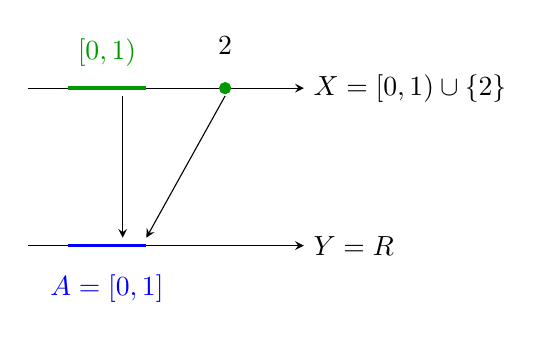
\begin{tikzpicture}[scale=1,>=stealth]
  % Eje del dominio
  \draw[->] (-0.5,0) -- (3,0) node[right] {$X=[0,1)\cup\{2\}$};
  % Intervalo [0,1)
  \draw[very thick,green!60!black] (0,0) -- (1,0);
  \node[above,green!60!black] at (0.5,0.15) {$[0,1)$};
  % Punto aislado 2
  \filldraw[green!60!black] (2,0) circle (2pt);
  \node[above] at (2,0.3) {$2$};

  % Eje del codominio
  \draw[->] (-0.5,-2) -- (3,-2) node[right] {$Y=\mathbb R$};
  % Intervalo A
  \draw[very thick,blue] (0,-2) -- (1,-2);
  \node[below,blue] at (0.5,-2.25) {$A=[0,1]$};

  % Flechas de la función
  \draw[->] (0.7,-0.1) -- (0.7,-1.9);  % para x en [0,1)
  \draw[->] (2,-0.1) -- (1,-1.9);      % para x=2
\end{tikzpicture}
\end{center}

\paragraph{\textbf{Ejemplo.}}
Sea $(X,\mathcal T_{\text{discreta}})$ el mismo conjunto $X$ con la topología discreta, y $(X,\mathcal T_{\text{trivial}})$ con la topología trivial.  
La identidad $\mathrm{id}\colon(X,\mathcal T_{\text{discreta}})\to(X,\mathcal T_{\text{trivial}})$ es continua.  
El espacio $(X,\mathcal T_{\text{trivial}})$ es conexo, mientras que $(X,\mathcal T_{\text{discreta}})$ no lo es si $|X|>1$.

\paragraph{\textbf{Definición.}}
Una aplicación $f\colon X\to Y$ es \emph{abierta} si envía abiertos en abiertos.  

%--------------------------------------------------
%  Producto de espacios conexos
%--------------------------------------------------

\subsection{Conexidad en la topología producto}

\paragraph{\textbf{Lema.}}
Sea $\{A_i\}_{i\in I}$ una colección de subespacios conexos de $X$ tal que
\begin{align*}
\bigcap_{i\in I}A_i\neq\varnothing .
\end{align*}
Entonces $\displaystyle\bigcup_{i\in I}A_i$ es conexo.

\paragraph{\textbf{Demostración.}}
Supongamos que
\begin{align*}
\bigcup_{i\in I}A_i=C\cup D
\end{align*}
es una separación con $C,D$ abiertos y disjuntos.  
Para todo $j\in I$,
\begin{align*}
A_j=(C\cap A_j)\cup(D\cap A_j),
\end{align*}
luego $A_j\subseteq C$ o $A_j\subseteq D$.  
Como la intersección común es no vacía, todos los $A_i$ quedan del mismo lado, contradicción. \hfill$\square$

\paragraph{\textbf{Teorema.}}
Si $X$ y $Y$ son espacios conexos, entonces:
\begin{enumerate}
  \item $(X\times\{y_0\})\cup(\{x_0\}\times Y)$ es conexo para cualquier $x_0\in X$ y $y_0\in Y$;
  \item $X\times Y$ es conexo.
\end{enumerate}

\paragraph{\textbf{Demostración.}}
\begin{enumerate}
  \item Cada conjunto $X\times\{y_0\}$ y $\{x_0\}\times Y$ es homeomorfo a $X$ y $Y$ respectivamente, de modo que ambos son conexos.  
        Su intersección contiene $(x_0,y_0)$; por el lema, la unión es conexa.
  \item Fijado $y_0\in Y$, escribimos
        \begin{align*}
        X\times Y=\bigcup_{x\in X}\Bigl[(X\times\{y_0\})\cup(\{x\}\times Y)\Bigr],
        \end{align*}
        donde cada término es conexo por (1) y la intersección de todos ellos contiene es no vacía, pues:
        \begin{align*}
          \bigcap_{x \in X} (X \times \{y_0\}) \cup (\{x\} \times Y)= X \times \{y_0\} 
        \end{align*}
        Por el lema anterior:
        \begin{align*}
          \bigcup_{y \in Y} \bigcup_{x \in X} (X \times \{y\}) \cup (\{x\} \times Y) = X \times Y
        \end{align*}
        Por lo tanto $X\times Y$ es conexo. \qedhere
\end{enumerate}

\paragraph{\textbf{Corolario.}}
Los siguientes espacios son conexos:
\begin{itemize}
  \item $\mathbb R^{n}$, pues $\mathbb R$ es conexo:
  \begin{align*}
    \mathbb R = \bigcup_{x\in \mathbb R^+}[-x,x]
  \end{align*}
  \item El intervalo cerrado $[a,b]$;
  \item El intervalo abierto $(a,b)$, pues
    \begin{align*}
      (a,b)=\bigcup_{\substack{a<c<\frac{a+b}{2} \\ \frac{a+b}{2}<d<b}} [c,d].
    \end{align*}
    \begin{center}
      \begin{tikzpicture}[>=stealth]
        % Real line with arrows
        \draw[<->] (-5,0) -- (5,0);
        % Endpoints a and b
        \coordinate (A) at (-3,0);
        \coordinate (B) at (3,0);
        \draw (A) -- ++(0,0.1) -- ++(0,-0.2) node[below] {$a$};
        \draw (B) -- ++(0,0.1) -- ++(0,-0.2) node[below] {$b$};
        % Midpoint
        \coordinate (M) at ($(A)!0.5!(B)$);
        \draw (M) -- ++(0,0.1) -- ++(0,-0.2) node[below] {$\frac{a+b}{2}$};
        % Points c and d near midpoint
        \coordinate (C) at ($(A)!0.4!(B)$);
        \draw (C) -- ++(0,0.1) -- ++(0,-0.2) node[above] {$c$};
        \coordinate (D) at ($(A)!0.6!(B)$);
        \draw (D) -- ++(0,0.1) -- ++(0,-0.2) node[above] {$d$};
      \end{tikzpicture}
    \end{center}
    \item $B_1(0,0)$ es conexo, pues 
\begin{center}
\begin{tikzpicture}[>=stealth,scale=1]
  % Unit circle with axes
  \draw[->] (-1.5,0) -- (1.5,0) node[right] {$x$};
  \draw[->] (0,-1.5) -- (0,1.5) node[above] {$y$};
  \draw (0,0) circle (1cm);
  % Isomorphism symbol
  \node at (3,0) {$\cong$};
  % Square [0,1]x[0,1]
  \draw (5,0) rectangle ++(1,1);
  \draw[->] (-1.5+5,0) -- (1.5+5,0) node[right] {$x$};
  \draw[->] (5,-1.5) -- (5,1.5) node[above] {$y$};
  \node at (6.2,-0.5) {$[0,1]\times[0,1]$};
\end{tikzpicture}
\end{center}
    
\end{itemize}

%--------------------------------------------------
%  Conexión por caminos
%--------------------------------------------------

\subsection{Conexidad por caminos}

\paragraph{\textbf{Definición.}}
Un espacio topológico $X$ es \emph{arco conexo} (o \emph{conexo por caminos}) si para cualesquiera $x,y\in X$ existe un camino continuo $\gamma\colon[0,1]\to X$ con $\gamma(0)=x$ y $\gamma(1)=y$.

\begin{center}
  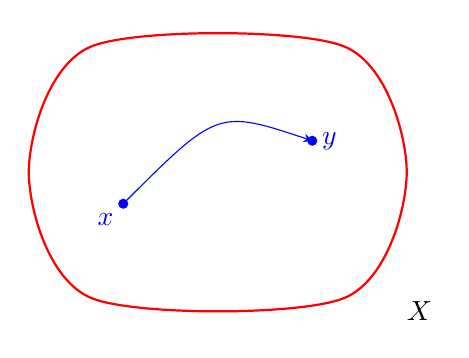
\begin{tikzpicture}[>=stealth,scale=0.8]
    % Región X
    \draw[red, thick, smooth cycle]
      plot coordinates {(-3,0) (-2,2) (2,2) (3,0) (2,-2) (-2,-2)};
    \node at (3.2,-2.2) {$X$};
    % Puntos x y y
    \coordinate (xpt) at (-1.5,-0.5);
    \coordinate (ypt) at (1.5,0.5);
    \filldraw[blue] (xpt) circle (2pt) node[below left] {$x$};
    \filldraw[blue] (ypt) circle (2pt) node[right] {$y$};
    % Camino de x a y
    \draw[blue,->] (xpt) .. controls (0,1) .. (ypt);
  \end{tikzpicture}
  \end{center}
  

\paragraph{\textbf{Teorema.}}
Si $X$ es arco conexo, entonces $X$ es conexo.

\paragraph{\textbf{Demostración.}}
Fijemos $x_0\in X$.  
Para cada $x\in X$ existe un camino $\gamma_x$ que une $x_0$ con $x$.  
Cada imagen $\operatorname{Im}(\gamma_x)$ es conexa y
\begin{align*}
X=\bigcup_{x\in X}\operatorname{Im}(\gamma_x),
\end{align*}
mientras que $x_0$ pertenece a todas ellas.  
Por el lema anterior, $X$ es conexo. \hfill$\square$

\paragraph{\textbf{Ejercicio.}}
Demuestre que $(0,\infty)$ es conexo.

%--------------------------------------------------
%  La curva del topólogo
%--------------------------------------------------

\subsection{La curva del topólogo}

Sea $f(x)=\sin\!\bigl(\tfrac1x\bigr)$ para $x>0$ y defina $F(x)=(x,f(x))$.  
Sea
\begin{align*}
C=\Gamma_F=\Bigl\{\bigl(x,\sin\tfrac1x\bigr):x\in(0,\infty)\Bigr\}.
\end{align*}


\begin{center}
  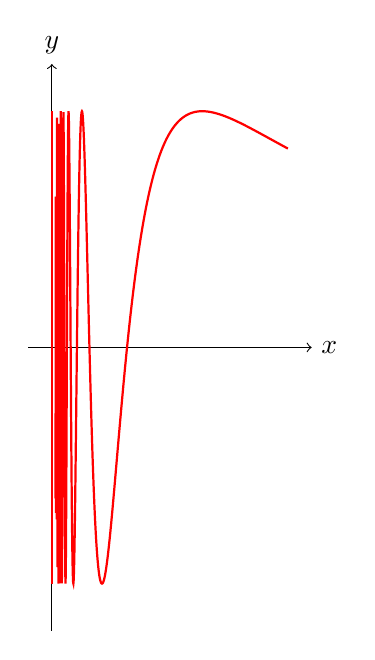
\begin{tikzpicture}[scale=3]
    % Axes
    \draw[->] (-0.1,0) -- (1.1,0) node[right] {$x$};
    \draw[->] (0,-1.2) -- (0,1.2) node[above] {$y$};
    % Graph of sin(1/x) for x>0
    \draw[red, thick, domain=0.015:1, samples=1000] plot (\x,{sin(deg(1/\x))});
    % Closure segment at x=0
    \draw[red, thick] (0,-1) -- (0,1);
  \end{tikzpicture}
  \end{center}
  

\begin{itemize}
  \item $C$ es arco conexo, pues para cada $x,y\in C$ existe un camino sobre la curva que une $x$ y $y$;
  \item $C$ es conexo, pues $C$ es arco conexo;
  \item $\overline{C}$ es conexo (Lema pagina 23 Hatcher);
  \item $\overline{C}$ no es arco conexo.
\end{itemize}

Obsérvese que $\overline{C}=C\cup\bigl(\{0\}\times[-1,1]\bigr)$.  
El punto $(0,1)$ no puede unirse mediante un camino dentro de $\overline{C}$ con $\bigl(\tfrac2\pi,1\bigr)$: cualquier trayecto continuo queda atrapado en $\{0\}\times[-1,1]$ durante un intervalo inicial de tiempo, impidiendo alcanzar el punto mencionado.
%  Fin de la clase 6
%--------------------------------------------------